\documentclass[12pt]{report}

\usepackage{amssymb, fullpage, amsmath}
\usepackage{graphicx}


\def\Xint#1{\mathchoice
   {\XXint\displaystyle\textstyle{#1}}%
   {\XXint\textstyle\scriptstyle{#1}}%
   {\XXint\scriptstyle\scriptscriptstyle{#1}}%
   {\XXint\scriptscriptstyle\scriptscriptstyle{#1}}%
   \!\int}
\def\XXint#1#2#3{{\setbox0=\hbox{$#1{#2#3}{\int}$}
     \vcenter{\hbox{$#2#3$}}\kern-.5\wd0}}
\def\ddashint{\Xint=}
\def\dashint{\Xint-}

\newtheorem{problem}{Problem}

\newenvironment{solution}[1][\it{Solution}]{\textbf{#1. } }{$\square$}

\graphicspath{ {./} }

\pagestyle{empty}

\def\Z{{\mathbb Z}}
\def\Q{{\mathbb Q}}
\def\C{{\mathbb C}}
\def\R{{\mathbb R}}
\def\N{{\mathbb N}}
\def\O{{\mathcal{O}}}

\def\dashint{\Xint-}

\begin{document}

\large

\begin{center}
 Math 573 Homework 2\\
 Due October 21\\
 By Marvyn Bailly\\
\end{center}

\normalsize

\hrule

%---------------%
%---Problem 1---%
%---------------%

%--status--$

\begin{problem}
    {\bf The Benjamin-Ono equation}
    \[
    u_t+u u_x+{\cal H}u_{xx}=0
    \]
    is used to describe internal waves in deep water. Here ${\cal H}f(x,t)$ is the spatial Hilbert transform of
    $f(x,t)$:
    \[
    {\cal H}f(x,t)=\frac{1}{\pi}\dashint_{-\infty}^\infty \frac{f(z,t)}{z-x}dz,
    \]
    and $\dashint$ denotes the Cauchy principal value integral. Write down the linear
    dispersion relationship for this equation linearized about the zero solution.
    
\end{problem}

\begin{solution}
    \noindent
    (Worked with Kaitlynn and Damien)

    \noindent
    Consider the Benjamin-Ono equation,
    \begin{align}
        u_t+u u_x+{\cal H}u_{xx}=0
    \end{align}
    where ${\cal H}f(x,t)$ is the spatial Hilbert transform of
    $f(x,t)$:
    \[
    {\cal H}f(x,t)=\frac{1}{\pi}\int_{-\infty}^\infty \frac{f(z,t)}{z-x}dz.
    \]
    Let's begin by linearizing. Assume that $u \rightarrow a$ as $|x| \rightarrow \infty$ and let $$u = a + \epsilon \nu + \O(\epsilon^2)$$
    where $\epsilon$ is a small parameter. Plugging this solution into (1),
    \[
    \epsilon \nu_t + (a + \epsilon\nu)\nu_x + {\cal H} \epsilon \nu_xx + \O(\epsilon^2) = 0.
    \]
    Collecting the first order $\epsilon$ terms we get,
    \[
    \nu_t + a \nu_x + {\cal H}v_{xx} = 0.
    \]
    Since we know that $0$ is a solution, let's linearize around $a = 0$ which gives,
    \begin{align}
        \nu_t + {\cal H}v_{xx} = 0.
    \end{align}
    Let's assume that $\nu$ is of the form,
    \[
    \nu = e^{i k x - i \omega t}
    \]
    plugging $\nu$ into (2) we have,
    \begin{align}
        -i\omega e^{i k x - i \omega t} +   {\cal H} (ik)^2 e^{i k x - i \omega t} &= 0
    \end{align}
    Evaluating ${\cal H}(e^{i k x - i \omega t})$ gives,
    \[
        {\cal H}(e^{i k x - i \omega t}) = \frac{-k^2}{\pi}\int_{-\infty}^{\infty} \frac{e^{ikz - iwt}}{z - x}dz
    \]
    if we let $\xi = z -x$ then,
    \[
        \frac{-k^2}{\pi}\int_{-\infty}^{\infty} \frac{e^{ik(\xi + x) - i\omega t}}{\xi}d\xi = \frac{-k^2}{\pi} e^{ikx - i\omega t} \int_{-\infty}^{\infty} \frac{e^{ik\xi}}{\xi}d\xi.
    \]
    Without loss of generality, assume that $k > 0$. The contour of this integral has one singularity that we are approaching on both sides by $\epsilon$. The lines also both go out to $\pm R$. We can connect these lines with a semi circle that goes above the singularity and call it $C_\epsilon$. We can also connect the end points of each line with a semi circle $C_R$. Thus we can rewrite the integral as,
    \[
        \oint_C \frac{e^{ik\xi}}{\xi}d\xi = \left( \int_{-R}^{-\epsilon} + \int_{R}^{\epsilon}\right) \frac{e^{ik\xi}}{\xi}d\xi + \int_{C_\epsilon} \frac{e^{ik\xi}}{\xi}d\xi + \int_{C_R}\frac{e^{ik\xi}}{\xi}d\xi = 0
    \] 
    since we assumed $k > 0$, the integral satisfies Jordan's Lemma and thus vanishes as $R \rightarrow \infty$. We also noted that there is a singularity which is a simple pole and therefore $\lim_{\epsilon \rightarrow 0}\int_{C_\epsilon} \frac{e^{ik\xi}}{\xi}d\xi = -i \pi$ where the minus is due to the integral being in a clockwise direction. Thus as $R \rightarrow \infty$ we have,
    \[
        \oint_C \frac{e^{ik\xi}}{\xi}d\xi = \int_{-\infty}^{\infty} \frac{\cos(k\xi)}{\xi}d\xi + i\int_{-\infty}^{\infty} \frac{\sin(k\xi)}{\xi}d\xi = i\pi.
    \]    
    Note that the same result would be obtained when $k < 0$ when evaluating the above integral due to the $\sin$ and $\cos$ terms. Putting this result back into (3) we get,
    \begin{align*}
        -i\omega e^{i k x - i \omega t} + (ik)^2  \left( \frac{-k^2}{\pi} e^{ikx - i\omega t} \right)(i \pi) &= 0\\
        -i\omega e^{i k x - i \omega t} +  -ik^2 e^{ikx - i\omega t} &= 0\\
        -i\omega - ik^2 &= 0\\
        \omega &= -k^2\\
    \end{align*}
    and we have found that the dispersion relation is given by $\omega = -k^2$.
\end{solution}

%----------------------------------------------------------------------------------------------------%
%\vskip 20pt
\newpage

%---------------%
%---Problem 2---%
%---------------%

%--talk more about Taylor--$

\begin{problem}
    Derive the linear dispersion relationship for the one-dimensional
surface water wave problem by linearizing around the trivial solution $\zeta(x,t)=0$, $\phi(x,z,t)=0$:
\begin{eqnarray*}
\nabla^2\phi=0,&& ~~~~-h<z<\zeta(x,t)\\
\phi_z=0, && ~~~~ z=-h\\
\zeta_t+\phi_x\zeta_x=\phi_z, && ~~~~z=\zeta(x,t)\\
\phi_t+g\zeta+\frac{1}{2}\left(\phi_x^2+\phi_z^2\right)=
T\frac{\zeta_{xx}}{\left(1+\zeta_x^2\right)^{3/2}}, && ~~~~z=\zeta(x,t)
\end{eqnarray*}
Here $z=\zeta(x,t)$ is the surface of the water,
$\phi(x,z,t)$ is the velocity potential so that $v=\nabla \phi$ is the velocity of the water, $g$ is
the acceleration of gravity, and $T>0$ is the coefficient of surface tension.
\end{problem}

\begin{solution}
    (Worked with Kaitlynn)

    \noindent
    Consider linear dispersion relationship for the one-dimensional
    surface water wave Problem $\zeta(x,t)=0$, $\phi(x,z,t)=0$:
    \begin{eqnarray*}
    \nabla^2\phi=0,&& ~~~~-h<z<\zeta(x,t)\\
    \phi_z=0, && ~~~~ z=-h\\
    \zeta_t+\phi_x\zeta_x=\phi_z, && ~~~~z=\zeta(x,t)\\
    \phi_t+g\zeta+\frac{1}{2}\left(\phi_x^2+\phi_z^2\right)=
    T\frac{\zeta_{xx}}{\left(1+\zeta_x^2\right)^{3/2}}, && ~~~~z=\zeta(x,t)
    \end{eqnarray*}
    where $z=\zeta(x,t)$ is the surface of the water,
    $\phi(x,z,t)$ is the velocity potential so that $v=\nabla \phi$ is the velocity of the water, $g$ is
    the acceleration of gravity, and $T>0$ is the coefficient of surface tension. 
    
    \noindent
    Let's begin by linearizing. Assume that $\zeta \rightarrow u$ as $|z| \rightarrow \infty$ and $\phi \rightarrow v$ as $|z| \rightarrow \infty$ to get,
    \begin{align*}
        \zeta &= \alpha + \epsilon u + \O(\epsilon^2)\\
        \phi &= \beta + \epsilon v + \O(\epsilon^2)
    \end{align*}
    where $\epsilon$ is a small parameter. This gives us the system,
    \begin{eqnarray*}
    \nabla^2(\beta + \epsilon v) +  \O(\epsilon^2)=\epsilon(v_{xx} + v_{yy})+ \O{\epsilon} = 0,&& ~~~~-h<z<\alpha + \epsilon u + \O(\epsilon^2)\\
    \epsilon v_{z} + \O(\epsilon^2)=0, && ~~~~ z=-h\\
    \epsilon u_t + (\epsilon v_x)(\epsilon u_X) = \epsilon v_x + \O(\epsilon^2), && ~~~~z=\alpha + \epsilon u + \O(\epsilon^2)\\
    \epsilon v_t + g(\alpha + \epsilon u) + \frac{1}{2}((\epsilon v_x)^2+(\epsilon v_z)^2) = T \frac{\epsilon u_{xx}}{\left(1+(\epsilon u+x)^2\right)^\frac{3}{2}}, && ~~~~z=\alpha + \epsilon u + \O(\epsilon^2)
    \end{eqnarray*}
    Taking the first order terms and linearizing around the trivial solution $\alpha = \beta = 0$ we get,
    \begin{eqnarray*}
        \nabla^2 v = 0,&& ~~~~-h<z<0\\
        v_{z} =0, && ~~~~ z=-h\\
        u_t = v_z, && ~~~~z=0\\
        v_t + gu = T u_{xx}, && ~~~~z=0
    \end{eqnarray*}
    where the bounds are zero by Taylor Expanding to the first term (since higher order terms will not be first order) and noticing it is equal to zero. Now if we let $v$ be a solution of the form $v = P(z)\cos(kx - \omega t)$ we have, 
    \begin{eqnarray}
        -k^2 P(z) \cos(kx - wt) + P''(z)\cos(kx - wt) = 0,&& ~~~~-h<z<0\\
        P'(z)\cos(kx - wt) =0, && ~~~~ z=-h\\
        u_t = v_z, && ~~~~z=0\\
        v_t + gu = T u_{xx}, && ~~~~z=0
    \end{eqnarray}
    Simplifying (4) we have the ODE $-k^2 P(z) + P''(z) = 0$ and using the boundary condition we get,
    \[ P = P_0 \cosh k(z + h).\] 
    were $P_0$ is an undetermined coefficient. We can verify this solution by plugging it into (5) which gives,
    \begin{align*}
        P'(z)\cos(kx - wt) &= 0,  ~~~~ z=-h\\
        kP_0\cos(kx - wt)\sinh k(z+ h) &= 0 ~~~~ z=-h\\
        kP_0\cos(kx - wt)\sinh 0 &= 0
    \end{align*}
    Thus $v = P_0 \cosh k(z + h)\cos(kx - \omega t)$. Assuming that $u$ is a solution of the form $u = Q(z)\sin(kx - \omega t)$, we can plug $u$ into (6) to get,
    \begin{align*}
         - \omega Q(z)\cos(kx - \omega t) &= k P_0 \sinh k(z + h)\cos(kx-\omega t)\\
        -\omega Q(z) &= k P_0 \sinh k(z + h)\\
        Q(z) &= -\frac{kP_0}{\omega}\sinh k(z + h)
    \end{align*}
    Thus $u = -\frac{kP_0}{\omega}\sinh k(z + h)\sin(kx - \omega t)$. Plugging $u$ and $v$ into (7) we can solve for $\omega$,
    \begin{align*}
        \omega P_0 \cosh k(z + h)\sin(kx - \omega t) + g(-\frac{kP_0}{\omega}\sinh k(z + h)\sin(kx - \omega t)) &= T(\frac{k^3P_0}{\omega}\sinh k(z + h)\sin(kx - \omega t))\\
        \omega \cosh k(z + h)  -\frac{gk}{\omega}\sinh k(z + h) &= T\frac{k^3}{\omega}\sinh k(z + h)\\
        \omega \cosh k(z + h)  &= \left( T\frac{k^3}{\omega} + \frac{gk}{\omega}\right)\sinh k(z + h)\\
        \omega^2 &= \left( Tk^3 + gk\right)\frac{\sinh k(z + h)}{\cosh k(z + h)}
    \end{align*}
    And thus $\omega^2 = \left( Tk^2 + gk \right)\tanh{k(z +h)}$ and when $z=0$ we have $\omega^2 = \left( Tk^2 + gk \right)\tanh{kh}$. Note that when we assume that there is no surface tension, the dispersion simplifies to $\omega^2 = gk \tanh kh$ as desired in question 3. 
\end{solution}

%----------------------------------------------------------------------------------------------------%
%\vskip 20pt
\newpage

%---------------%
%---Problem 3---%
%---------------%

%--status--$

\begin{problem}
    Having found that for the surface water wave problem without surface
tension the linear dispersion relationship is $\omega^2=gk\tanh(kh)$, find the
group velocities for the case of long waves in shallow water ($kh$ small), and
for the case of deep water ($kh$ big).
\end{problem}

\begin{solution}
    
    
    \noindent
    In question 2 we found that the surface water wave problem without surface
    tension has a linear dispersion relationship of $\omega^2=gk\tanh(kh)$ where $g$ is the acceleration of gravity. First let's find the group velocities for the case of long waves in shallow water. This occurs when $kh$ is small. To approximate small values of $kh$, we can Taylor expand $\tanh(kh) = kh - \frac{(kh)^3}{3} + \cdots$, and take the first term. Thus we have $\tanh(kh) \approx kh$ for small values of $kh$. Thus the dispersion relationship simplifies to $\omega = \sqrt{(gk)(hk)} = \sqrt{ghk^2}$. We know that the group velocity is defined by \[c_g = \frac{d\omega}{dk}\] and therefore the group velocity is,
    \begin{align*}
        c_g &= \sqrt{gh}.
    \end{align*} 
    Next we want to find the group velocity in deep water meaning that $kh$ is large. To approximate $\tanh(kh)$ when it is large, consider the exponential form,
    \begin{align*}
        \left( \frac{e^{kh} - e^{-kh}}{e^{kh} + e^{-kh}} \right) \left( \frac{e^{-kh}}{e^{-kh}}\right) = \frac{1-e^{2kh}}{1+e^{2kh}}\\
    \end{align*}
    Then we can take the limit as $kh$ gets big,
    \[
        \lim_{kh \rightarrow \infty} \tanh(kh) = \lim_{kh \rightarrow \infty} \frac{1 - e^{2kh}}{1 + e^{2kh}} = \frac{1}{1} = 1\\
    \]
    Therefore we can approximate large values  as $\tanh(kh) \approx 1$ giving us $\omega = \sqrt{gk}$ and thus the group velocity for large waves is given by $c_g = \frac{\sqrt{a}}{2\sqrt{k}}$
\end{solution}

%----------------------------------------------------------------------------------------------------%
%\vskip 20pt
\newpage

%---------------%
%---Problem 4---%
%---------------%

%--status--$

\begin{problem}
    Whitham wrote down what is now known as {\bf the Whitham equation} to incorporate the full effect of water-wave dispersion for waves in shallow water by modifying the KdV equation $u_t+vu_x+u u_x+\gamma u_{xxx}=0$ (where we have included the transport term) to

    \[
    u_t+uu_x+\int_{-\infty}^\infty K(x-y)u_y(y,t)dy=0,
    \]

    where
    \[
    K(x)=\frac{1}{2\pi}\dashint_{-\infty}^\infty c(k)e^{ikx}dk,
    \]

    and $c(k)$ is the positive phase speed for the water-wave problem: $c(k)=\sqrt{g\tanh(kh)/k}$.

    \begin{enumerate}

    \item What is the linear dispersion relation of the Whitham equation?

    \item Show that the dispersion relation of the KdV equation is an approximation to that of the Whitham equation for long waves, {\em i.e.}, for $k \rightarrow 0$. What are $v$ and $\gamma$?

    \end{enumerate}

    Note that using this process of ``Whithamization'', one could construct a KdV-like equation ({\em i.e.}, an equation with the KdV nonlinearity) that has any desired dispersion relation. Similar procedures can be followed for other equations, like the NLS equation {\em etc}.

\end{problem}

\begin{solution}
    (Worked with Kaitlynn and Annie)

    \noindent
    Consider the Whitham equation \[
        u_t+uu_x+\int_{-\infty}^\infty K(x-y)u_y(y,t)dy=0,
        \]
        where
        \[
        K(x)=\frac{1}{2\pi}\dashint_{-\infty}^\infty c(k)e^{ikx}dk,
        \]
        and $c(k)$ is the positive phase speed for the water-wave problem: $c(k)=\sqrt{g\tanh(kh)/k}$.
        \begin{enumerate}
            \item First let's find the linear dispersion relation.
            Let's begin by linearizing. Assume that $u \rightarrow a$ as $|x| \rightarrow \infty$  and let 
            \[ u = \alpha + \epsilon v + \O(\epsilon^2). \]
            Plugging this into the Whitham equation we get,
            \begin{align*}
                0 &= \epsilon v_t + (\alpha + \epsilon v)(\epsilon v_x) + \int_{-\infty}^{\infty}K(x-y)(\epsilon v_y)dy + \O(\epsilon^2)\\
                &= \epsilon v_t + \alpha\epsilon v_x + \epsilon^2vv_x + \int_{-\infty}^{\infty}K(x-y)(\epsilon v_y)dy + \O(\epsilon^2)\\
            \end{align*}
            Taking the first order terms we get,
            \[
                v_t + \alpha v_x + \int_{-\infty}^{\infty} K(x-y)v_y dy = 0
            \]
            If we linearize around the trivial solution $\alpha = 0$ then
            \begin{align*}
                0 &= v_t + \int_{-\infty}^{\infty} K(x-y)v_y dy\\
                &= v_t + \int_{-\infty}^{\infty} \frac{1}{2\pi} \dashint_{-\infty}^{\infty}c(l)e^{il(x-y)}dk v_y dy\\
                &= v_t + \int_{-\infty}^{\infty} \frac{1}{2\pi} \dashint_{-\infty}^{\infty}c(l)e^{il(x-y)}dk v_y dy\\
                &= v_t + \int_{-\infty}^{\infty} \frac{1}{2\pi} \dashint_{-\infty}^{\infty}\sqrt{g\tanh(lh)/l}e^{il(x-y)}dl v_y dy\\
            \end{align*}
            where $l$ is a dummy variable to avoid confuse between variables. Now let's assume that $v$ is a solution of the form $v = e^{ikx - iwt}$, this give
            \begin{align*}
                0 &= -i\omega e^{ikx - iwt} + \int_{-\infty}^{\infty} \frac{1}{2\pi} \dashint_{-\infty}^{\infty}\sqrt{g\tanh(lh)/l}e^{il(x-y)}dl (ike^{iky - iwt}) dy\\
                &= -i\omega e^{ikx - iwt} + \frac{ike^{-iwt}}{2\pi} \int_{-\infty}^{\infty} e^{iky} dy \dashint_{-\infty}^{\infty}e^{il(x-y)}\sqrt{g\tanh(lh)/l}dl \\
                &= -i\omega e^{ikx} + \frac{ik}{2\pi} \dashint_{-\infty}^{\infty} e^{ilx}\sqrt{g\tanh(lh)/l}dl \int_{-\infty}^{\infty}e^{iky}e^{-ily}\\
                &= -i\omega e^{ikx}+ ik \dashint_{-\infty}^{\infty} e^{ilx}\sqrt{g\tanh(lh)/l}dl \frac{1}{2\pi} \int_{-\infty}^{\infty}e^{i(k-l)i}
            \end{align*}
            Noticing that we have $\delta(k - l)$, the express simplifies to
            \begin{align*}
                 0 &= -i\omega e^{ikx} + (ik)e^{ikx}\sqrt{g\tanh(kh)/k}\\
                 &= -\omega + k \sqrt{g\tanh(kh)/k}\\
            \end{align*}
            and thus we have found the dispersion relation to be $\omega = \sqrt{gk\tanh(kh)}$.
            \item Next we wish to show that the dispersion relation of the KdV equation is an approximation to that of the Whitham equation. First let's linearize the KdV equation around the trival solution $0$. Assuming that $u \rightarrow 0$ as $|x| \rightarrow \infty$ and letting \[ u = \epsilon w + \O(\epsilon^2),\]
            were $\epsilon$ is a small parameter, we get that
            \[
                \epsilon w_t + v \epsilon w_x + \epsilon w(\epsilon w_x) + \gamma \epsilon w_{xxx} + \O(\epsilon^2) = 0.
            \]
            Taking the first order $\epsilon$ values we get,
            \[
                w_t + vw_x + \gamma w_{xxx} = 0.
            \]
            Assuming that $w$ is a solution of the form $w = e^{ikx - iwt}$ and plugging this into our equation we have,
            \begin{align*}
                0 &= -iwe^{ikx - iwt} + v (ik)e^{ikx - iwt} - \gamma ik^2 e^{ikx - iwt}\\
                &= -iw + vik + \gamma ik^3
            \end{align*}      
            and thus we have the dispersion relation to be $w(k) = vk - \gamma k^3$. 
            
            \noindent
            Now recall that the dispersion relation for the KdV equation is given by $\omega = \sqrt{gk\tanh(kh)}$. Since we want to show that the KdV dispersion relation can approximate that of the Whitham for small $k$ values, let's Taylor expand $\omega$ as,
            \[ 
                \omega^2 = gk\tanh(kh) = gk(kh - \frac{1}{3}(kh)^3 + \cdots) \]
            and taking the first two terms we get that, $\omega^2 \approx gk(kh - \frac{1}{3}(kh)^2) = ghk^2(1 - \frac{1}{3}(kh)^2)$ as $k \rightarrow 0$. Therefore $\omega \approx \sqrt{gh}k(1 - \frac{1}{6}k^2) = \sqrt{gh} k - \frac{1}{6} \sqrt{gh}k^3$. Thus $v = \sqrt{gh}$ and $\gamma = \frac{1}{6} \sqrt{gh}$. 
        \end{enumerate}
\end{solution}

%----------------------------------------------------------------------------------------------------%
%\vskip 20pt
\newpage

%---------------%
%---Problem 5---%
%---------------%

%--status--$

\begin{problem}
    Consider the linear free Schr\"odinger (``free'', because there's no
potential) equation
$$
i \psi_t+\psi_{xx}=0, ~~~~~-\infty<x<\infty,~~t>0, ~~\psi\rightarrow 0
~~\mbox{as}~~ |x|\rightarrow \infty,
$$
with $\psi(x,0)=\psi_0(x)$ such that $\int_{-\infty}^\infty|\psi_0|^2
dx<\infty$.

\begin{enumerate}

\item Using the Fourier transform, write down the solution of this problem.

\item Using the Method of Stationary Phase, find the dominant behavior as
$t\rightarrow \infty$ of the
solution, along lines of constant $x/t$.

\item With $\psi_0(x)=e^{-x^2}$, the integral can be worked out exactly.
Compare (graphically or other) this exact answer with the answer you get from
the Method of Stationary Phase. Use the lines $x/t=1$ and $x/t=2$ to compare.

\item Use your favorite numerical integrator (write your own, or use maple,
mathematica or matlab) to compare (graphically or other) with the exact answer
and the answer you get from the Method of Stationary Phase.

\end{enumerate}
\end{problem}

\begin{solution}
    (Worked with Kaitlynn, Annie, Damien, Cade, and Bernard)

    \noindent
    Consider the linear free Schr\"odinger equation,
    \[
        i\psi_t + \psi_{xx} = 0, ~~~~~-\infty<x<\infty,~~t>0, ~~\psi\rightarrow 0
        ~~\mbox{as}~~ |x|\rightarrow \infty,
    \]
    with $\psi(x,0)=\psi_0(x)$ such that $\int_{-\infty}^\infty|\psi_0|^2
dx<\infty$.
    \begin{enumerate}
        \item First let's find the exact solution using Fourier Transforms. Recall that the Fourier is given by
        \[
            \hat{f}(\xi) = \int_{-\infty}^{\infty} f(x) e^{-i \xi x}dx ~~~ \forall \xi \in \R
        \]
        with,
        \[
            \mathcal{F} [f^{(n)}](\xi) = (i\xi)^n\hat{f}(\xi)
        \]
        Applying the Fourier transformation to the Linear Schr\"odinger equation,
        \begin{align*}
            i \frac{\partial}{\partial t} \hat{\psi}(\xi,t) + (i \xi)^2 \hat{\psi}(\xi,t) &= 0\\
            \implies i \hat{\psi}' - \xi^2 \hat{\psi} &= 0\\
            \implies \hat{\psi}' = \frac{\xi^2}{i}\hat{\psi}\\
            \implies \hat{\psi} = a(\xi) e^{-i\xi^2 t}
        \end{align*}
        Recall that the inverse of the Fourier Transformation is given by,
        \[ 
            f(x) = \frac{1}{2\pi} \int_{-\infty}^{\infty} \hat{f}(\xi)e^{i \xi x}d\xi
        \]
        which gives us that,
        \[
            \psi(x,t) = \frac{1}{2\pi} \int_{-\infty}^{\infty} a(\xi) e^{-i\xi^2 t}e^{i\xi x} d\xi
        \]
        which gives the exact solution to the Linear Schr\"odinger.

        \item Now let's apply the Stationary Phase Method. Since the free Schr\"odinger equation is already linear, let's begin by assuming that $\psi$ is a solution of the form $\psi = e^{ikx - i\omega t}$. Plugging this into the equation we get,
        \begin{align*}
            i(-i\omega)e^{ikx - i\omega t} - k^2 e^{ikx - i\omega t} &= 0\\
            \implies \omega = k^2
        \end{align*}
        To examine the long term asymptotics of $\psi$ consider,
        \[ \phi(k) = \frac{x}{t}k - \omega = \frac{x}{t}k - k^2\]
        which gives that $\phi'(k) = \frac{x}{t} - 2k$ and $\phi''(k) = -2$. Thus the Stationary points occur at \[k_0 = \frac{x}{2t}.\]  Plugging this into the given equation for Stationary Phase we gain,
        \begin{align*}
             \frac{a(k_0)}{\sqrt{2\pi t \phi''(k_0)}}e^{i\phi(k_0)t + i \pi \text{sgn}(\phi''(k_0))/4} &= \frac{a(k_0)}{\sqrt{4\pi t}}e^{i\phi(k_0)t + \frac{i\pi(-1)}{4}}\\
             &= \frac{a\left( \frac{x}{2t}\right)}{2\sqrt{\pi t}}e^{i \frac{x^2}{4t} - i \frac{\pi}{4}}
        \end{align*}
        which show us the dominant behavior as $t \rightarrow \infty$.
        
        \item With the initial condition $\psi_0(x) = e^{-x^2}$ we can solve for our equations from part 1 and 3. First let's solve for the exact solution. We have that
        \[
            \psi(x,0) = \frac{1}{2\pi}\int_{-\infty}^{\infty} a(\xi) e^{i\xi x}d\xi = e^{-x^2}
        \]  
        Combining this with $\hat{\psi}(\xi,0) = a(\xi)$ we can directly compute $a(\xi)$ by evaluating
        \[ a(\xi) = \int_{-\infty}^{\infty}e^{-x^2 - i\xi x}dx. \]
        Using Mathematica we get that $a(\xi) = \sqrt{\pi} e^{-\frac{\xi^2}{4}}$. Thus we have that,
        \[
            \psi(x,t) = \frac{1}{2\pi}\int_{-\infty}^{\infty} \sqrt{\pi} e^{-\frac{\xi^2}{4}} e^{-i\xi^2 t}e^{i\xi x} d\xi
        \] 
        and using Mathematica we get that the exact solution is,
        \begin{align}
            \psi(x,t) = \frac{e^{\frac{x^2}{-1-4it}}}{\sqrt{1 + 4it}}.
        \end{align}
        Next let's use $a(\xi)$ to find the Stationary Phase approximation,
        \begin{align*}
            \frac{a\left( \frac{x}{2t}\right)}{2\sqrt{\pi t}}e^{i \frac{x^2}{4t} - i \frac{\pi}{4}} = \frac{\sqrt{\pi}e^{-\frac{x^2}{16t^2}}}{2\sqrt{\pi t}}e^{i\frac{x^2}{4t} - i\frac{\pi}{4}}\\
        \end{align*}
        which simplifies to be,
        \begin{align}
            \frac{e^{-\frac{x^2}{16t^2} + i \frac{x^2}{4t} - i \frac{\pi}{4}}}{2\sqrt{t}}
        \end{align}
        Plotting (8) and (9) along the line $x/t = 1$ in Mathematica we get the two graphs in Figure \ref{fig:Figure 1}.
        \begin{figure}%
            \centering
            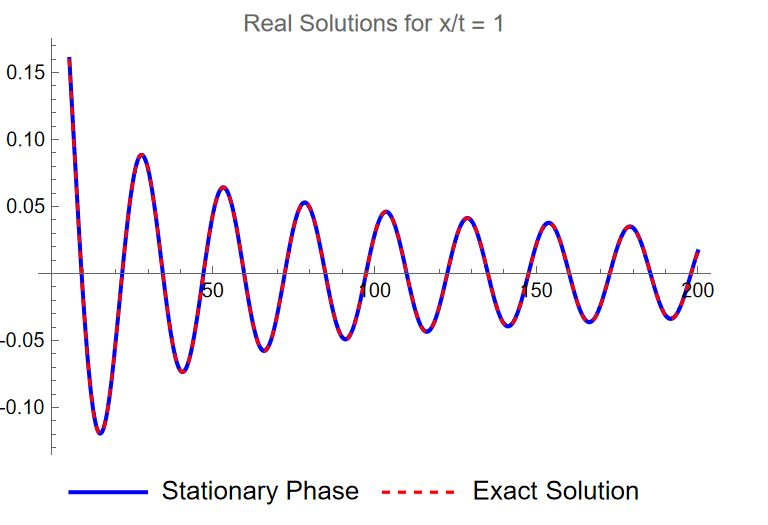
\includegraphics[width=.4\textwidth]{plots/realx1.JPG}
            \qquad
            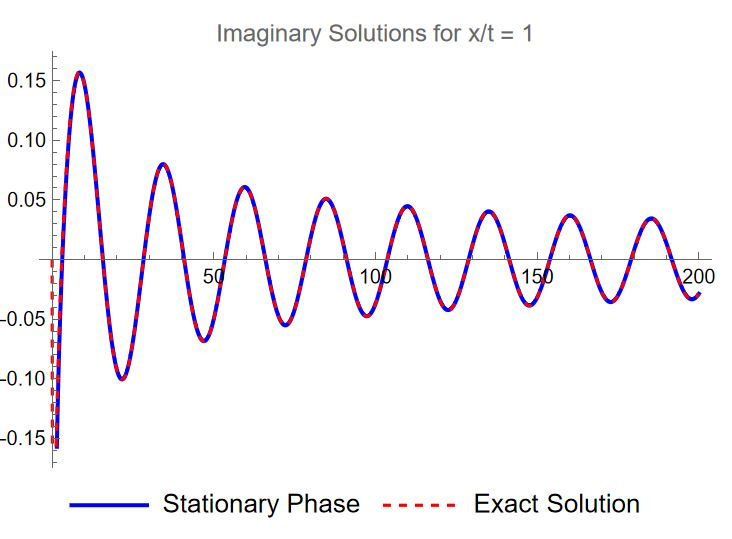
\includegraphics[width=.4\textwidth]{plots/fakex1.JPG}
            \caption{Real and Imaginary Solutions along the lines $x/t=1$ for Stationary Phase and Fourier methods}%
            \label{fig:Figure 1}%
        \end{figure}
        We can see that the solution derived from the Stationary Phase method match the exact solution very closely. It is also important to note that the computation time of Mathematica to compute the plots for the exact solution was significantly longer than that of the Stationary Phase solution. While these observations may be restricted to solutions with lower oscillations, we can plot (8) and (9) along the lines $x/t = 2$ which gives us Figure \ref{fig:Figure 2}.
        \begin{figure}%
            \centering
            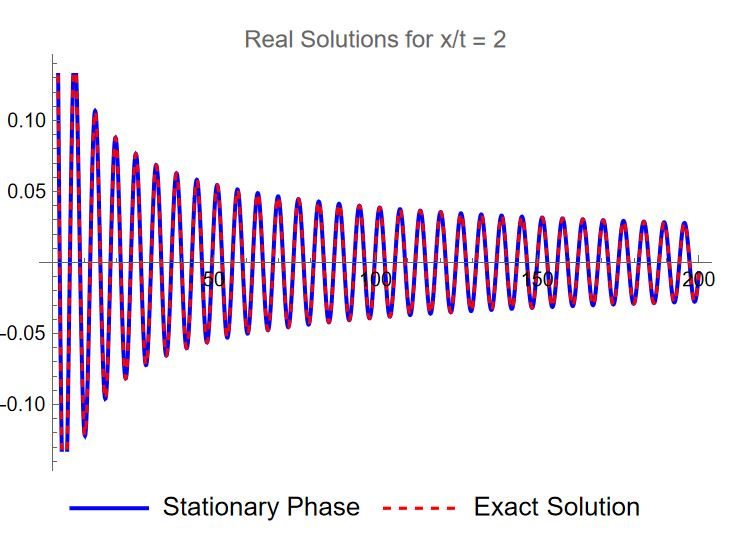
\includegraphics[width=.4\textwidth]{plots/realx2.JPG}
            \qquad
            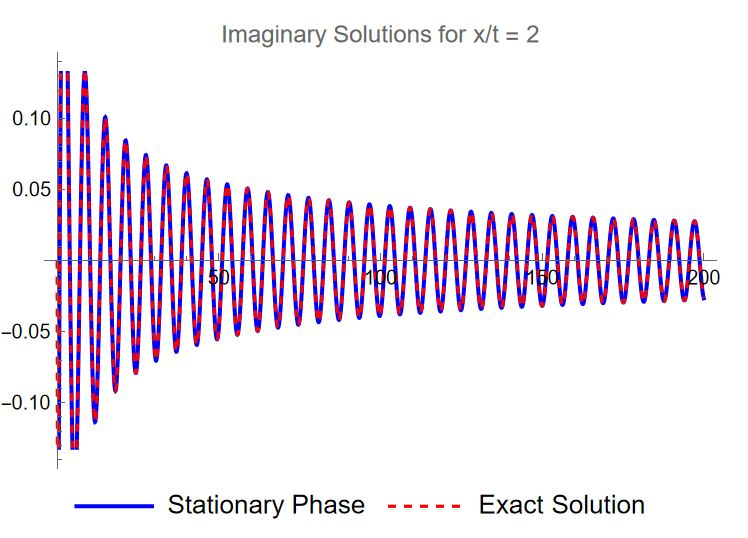
\includegraphics[width=.4\textwidth]{plots/fakex2.JPG}
            \caption{Real and Imaginary Solutions along the lines $x/t=2$ for Stationary Phase and Fourier methods}%
            \label{fig:Figure 2}%
        \end{figure} 
        Looking at these graphs we see that the Stationary Phase method still matches the exact solution very closely. Once again the stationary phase method computed significantly faster than the exact solution. Note that since the solutions are complex, I picked to plot their imaginary and real values individually. 

        \item Next we wish to compare the exact and stationary phase methods to a numerical integrator. I picked to use Mathematica's \verb+NIntegrate+ function to evaluate the integral, 
        \[
            \psi(x,t) = \frac{1}{2\pi}\int_{-\infty}^{\infty} \sqrt{\pi} e^{-\frac{\xi^2}{4}} e^{-i\xi^2 t}e^{i\xi x} d\xi.
        \] 
        Now with three different solutions, I plotted the real and imaginary parts using Mathematica to get the results in Figure 3.
        \begin{figure}%
            \centering
            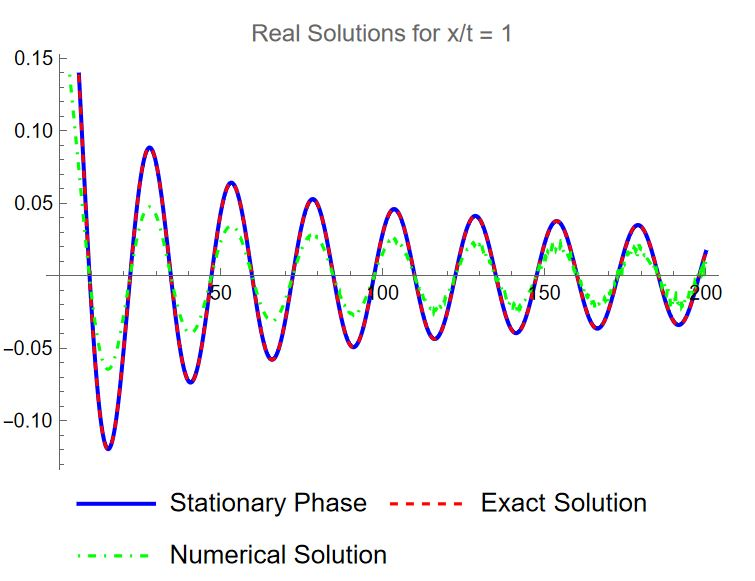
\includegraphics[width=.4\textwidth]{plots/realx3.JPG}
            \qquad
            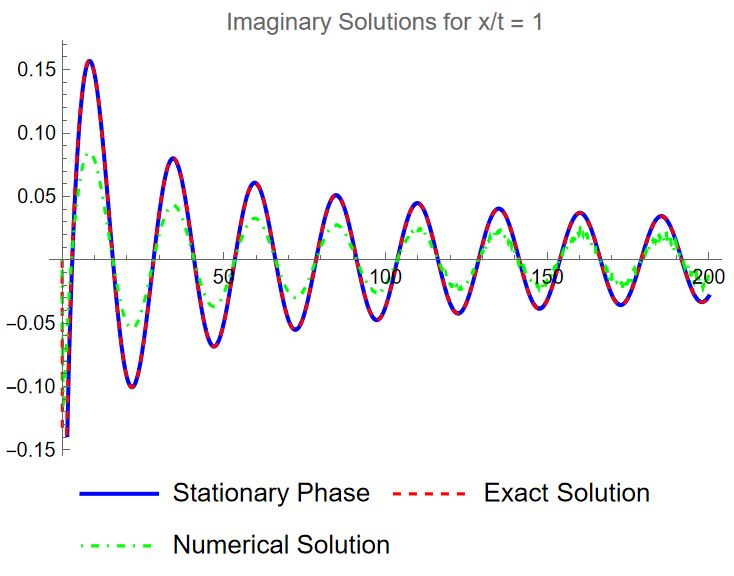
\includegraphics[width=.4\textwidth]{plots/fakex3.JPG}
            \caption{Real and Imaginary Solutions along the lines $x/t=1$ for Stationary Phase, Fourier, and Numerical methods}%
            \label{fig:Figure 3}%
        \end{figure} 
        We can see from the graphs that the numerical solution is notably inaccurate to the exact solution as the oscillations increase with $t$. In addition to the inaccuracy, the numerical solution took significantly longer to compute than the exact solution making it the slowest and most inaccurate of the three methods. Therefore the method of Stationary Phase is the best of the given methods to approximate long term (and seemingly short term) behavior of the Linear Schr\"odinger equation.
    \end{enumerate}
\end{solution}

%----------------------------------------------------------------------------------------------------%
%\vskip 20pt
\newpage

%---------------%
%---Problem 6---%
%---------------%

%--status--$

\begin{problem}
    Everything that we have done for continuous space equations also works
for equations with a discrete space variable. Consider the discrete linear
Schr\"odinger equation:
$$
i\frac{d\psi_n}{dt}+\frac{1}{h^2}(\psi_{n+1}-2 \psi_n+\psi_{n-1})=0,
$$
where $h$ is a real constant, $n$ is any integer, $t>0$, $\psi_n\rightarrow 0$
as $|n|\rightarrow \infty$, and $\psi_n(0)=\psi_{n,0}$ is given.
\begin{enumerate}
\item The discrete analogue of the Fourier transform is given by
$$
\psi_n(t)=\frac{1}{2\pi i}\oint_{|z|=1} \hat{\psi}(z,t) z^{n-1} dz,
$$
and its inverse
$$
\hat{\psi}(z,t)=\sum_{m=-\infty}^\infty \psi_m(t) z^{-m}.
$$
Show that these two transformations are indeed inverses of each other.
\item The dispersion relation of a semi-discrete problem is obtained by looking
for solutions of the form $\psi_n=z^n e^{-i \omega t}$. Show that for the
semi-discrete Schr\"odinger equation
$$
\omega(z)=-\frac{(z-1)^2}{zh^2}.
$$
How does this compare to the dispersion relation of the continuous space
problem? Specifically, demonstrate that you recover the dispersion relationship
for the continuous problem as $h\rightarrow 0$.
\end{enumerate}
\end{problem}

\begin{solution}
    (Worked with Kaitlynn and Ellie)

    \noindent
     
    Consider the discrete linear Schr\"odinger equation:
    $$
    i\frac{d\psi_n}{dt}+\frac{1}{h^2}(\psi_{n+1}-2 \psi_n+\psi_{n-1})=0,
    $$
    where $h$ is a real constant, $n$ is any integer, $t>0$, $\psi_n\rightarrow 0$
    as $|n|\rightarrow \infty$, and $\psi_n(0)=\psi_{n,0}$ is given.

    \begin{enumerate}
        \item First we wish to verify that the discrete analogue of the Fourier transform and its inverse are indeed inverses of each other. That is, $\mathcal{F} [ \mathcal{F}^{-1} \phi] = \phi$ and $\mathcal{F}^{-1} [ \mathcal{F} \phi] = \hat{\phi}$. Recall that the discrete analogue is given by 
        \[
        \psi_n(t)=\frac{1}{2\pi i}\oint_{|z|=1} \hat{\psi}(z,t) z^{n-1} dz,
        \]
        and its inverse
        \[
        \hat{\psi}(z,t)=\sum_{m=-\infty}^\infty \psi_m(t) z^{-m}.
        \].
        Let's begin by showing that $\mathcal{F} [ \mathcal{F}^{-1} \phi] = \phi$. Observe that,
        \begin{align*}
            \mathcal{F} [ \mathcal{F}^{-1} \phi] &= \mathcal{F} \left[ \sum_{m=-\infty}^\infty \psi_m(t) z^{-m} \right]\\
            &=\frac{1}{2\pi i}\oint_{|z|=1}z^{n-1}\sum_{m=-\infty}^\infty\psi_m(t)z^{-m}\mathrm{d}z\\
            &=\frac{1}{2\pi i}\sum_{m=-\infty}^\infty\psi_m(t)\oint_{|z|=1}z^{n-m-1}\mathrm{d}z.\\
        \end{align*}
        Using the transformation $z = Re^{i\theta}$ we get,
        \begin{align*}
            \mathcal{F}[\mathcal{F}^{-1}\psi]&=\frac{1}{2\pi i}\sum_{m=-\infty}^\infty\psi_m(t)\oint_0^{2\pi}(Re^{i\theta})^{n-m-1}(iRe^{i\theta})\mathrm{d}\theta\\
            &=\frac{1}{2\pi i}\sum_{m=-\infty}^\infty\psi_m(t)\oint_0^{2\pi}R^{n-m-1}e^{i(n-m-1)\theta}iRe^{i\theta}\mathrm{d}\theta\\
            &=\frac{1}{2\pi}\sum_{m=-\infty}^\infty\psi_m(t)R^{n-m}\oint_0^{2\pi}e^{i(n-m)\theta}\mathrm{d}\theta.\\
        \end{align*}
        To directly evaluate the integral, consider the two cases when $n = m$ and $n \neq m$. In the first case we have,
        \begin{align*}
            \mathcal{F}[\mathcal{F}^{-1}\psi]_{n=m}&=\frac{1}{2\pi}\sum_{m=-\infty}^\infty\psi_m(t)\oint_0^{2\pi}e^0\mathrm{d}\theta\\
            &=\frac{1}{2\pi}\sum_{m=-\infty}^\infty\psi_m(t)(2\pi)\\
            &=\sum_{m=-\infty}^\infty\psi_m(t)\\
            &=\psi.
        \end{align*}
        and in the latter case, we have
        \begin{align*}
            \mathcal{F}[\mathcal{F}^{-1}\psi]_{n\neq m}&=\frac{1}{2\pi}\sum_{m=-\infty}^\infty\psi_m(t)R^{n-m}\left[\frac{1}{i(n-m)}e^{i(n-m)\theta}\right]_0^{2\pi}\\
            &=\frac{1}{2\pi}\sum_{m=-\infty}^\infty\psi_m(t)R^{n-m}\left(\frac{1}{i(n-m)}\left(e^{i2\pi(n-m)}-1\right)\right)\\
            &=\frac{1}{2\pi}\sum_{m=-\infty}^\infty\psi_m(t)R^{n-m}(0)\\
            &=0.
        \end{align*}
        Combining these two cases, we get that the summation is,
        \begin{align*}
            \frac{1}{2\pi}\sum_{m=-\infty}^\infty\psi_m(t)R^{n-m}\oint_0^{2\pi}e^{i(n-m)\theta}\mathrm{d}\theta = \phi.\\
        \end{align*}
        and thus we have $\mathcal{F}[\mathcal{F}^{-1}\psi]=\psi$. Next we need to show the opposite direction, $\mathcal{F}^{-1}[\mathcal{F}\psi]=\hat{\psi}$. Observe that,
        \begin{align*}
            \mathcal{F}^{-1}[\mathcal{F}\psi]&=\mathcal{F}^{-1}\left[\frac{1}{2\pi i}\oint_{|z|=1}\hat{\psi}z^{n-1}\mathrm{d}z\right]\\
            &=\frac{1}{2\pi i}\sum_{m=-\infty}^\infty\left(\oint_{|z|=1}\hat{\psi}z^{m-1}\mathrm{d}z\right)z^{-m}.\\
        \end{align*}
        Recall that a Laurent Series is,
        \[f(z)=\sum_{n=-\infty}^\infty a_n(z-c)^n,\] 
        with 
        \[a_n=\frac{1}{2\pi i}\oint_\gamma\frac{f(z)}{(z-c)^{n+1}}\mathrm{d}z,\] 
        where $\gamma$ is the unit circle. To have our equation match the form of the Laurent Series, let $n = -m$ and observe that,
        \begin{align*}
            \mathcal{F}^{-1}[\mathcal{F}\psi]&=\frac{1}{2\pi i}\sum_{n=-\infty}^\infty\left(\oint_{|z|=1}\hat{\psi}z^{-n-1}\mathrm{d}z\right)z^{n}\\
            &=\sum_{n=-\infty}^\infty\left(\frac{1}{2\pi i}\oint_{|z|=1}\frac{\hat{\psi}}{z^{n+1}}\mathrm{d}z\right)z^n.\\
        \end{align*}
        Which is a Laurent Series where $c = 0$ and $f(z) = \hat{\psi}$. Thus we have that,
        \begin{align*}
            \sum_{n=-\infty}^\infty\left(\frac{1}{2\pi i}\oint_{|z|=1}\frac{\hat{\psi}}{z^{n+1}}\mathrm{d}z\right)z^n = \hat{\psi}
        \end{align*}
        which means that $\mathcal{F}^{-1}[\mathcal{F}\psi]=\hat{\psi}$. Therefore we have verified that the discrete analogue of the Fourier transform and its inverse are indeed inverses of each other.

        \item Next we wish to find the dispersion relation of the semi-discrete Shr\"odinger equation and show that we recover the dispersion relation for the continuous problem as $h \rightarrow 0$. Let's begin by finding the dispersion relation of the semi-discrete Shr\"odinger equation. Since the equation is already linear, we do not need to linearize. We are given that $\psi_n = z^n e^{i\omega t}$ and plugging this into the semi-discrete Shr\"odinger equation we get,
        \begin{align*}
            0 &= iz^n(-i\omega)e^{-i\omega t}+\frac{1}{h^2}(z^{n+1}e^{-i\omega t}-2z^ne^{-i\omega t}+z^{n-1}e^{-i\omega t})\\
            &=\omega z^n+\frac{1}{h^2}(z^{n+1}-2z^n+z^{n-1})\\
            &=\omega+\frac{1}{h^2z^n}(z^{n+1}-2z^n+z^{n-1})\\
            &=\omega+\frac{1}{h^2}(z-2+z^{-1})\\
            &=\omega+\frac{1}{h^2}\left(\frac{(z-1)^2}{z}\right)\\
            \Rightarrow \omega(z) &=-\frac{(z-1)^2}{zh^2},
        \end{align*}
        as expected. To find the relation between the dispersion relations, recall that,
        \[
            \lim_{n\rightarrow\infty}\left( 1 + \frac{a}{n}\right)^n = e^a
        \]
        where we will use the limit $n \rightarrow \infty$ to translate between the discrete and continuous equations. Notice that if we let $z = 1 + \frac{a}{n}$ and $a = ikx$ we get,
        \[
            \lim_{n\rightarrow\infty}\left( 1 + \frac{a}{n}\right)^n = \lim_{n \rightarrow \infty}z^n = e^{ikx}
        \] 
        which achieves the translation between the equations. Thus using $z = 1 + \frac{ikx}{n}$ and plugging it into the semi-discrete Shr\"odinger equation we have,
        \begin{align*}
            \omega(z)&=-\frac{(z-1)^2}{zh^2}\\
            &=-\frac{\left(1+\frac{ikx}{n}-1\right)^2}{\left(1+\frac{ikx}{n}\right)h^2}\\
            &=-\frac{\left(\frac{ikx}{n}\right)^2}{h^2+\frac{ikxh^2}{n}}\\
            &=\frac{\frac{k^2x^2}{n^2}}{h^2+\frac{ikxh^2}{n}}\\
            &=\frac{k^2x^2}{n^2h^2+iknxh^2}.
        \end{align*}
        and applying the transformation $x = nh$,
        \begin{align*}
            \omega(z)&=\frac{k^2(nh)^2}{n^2h^2+ikn(nh)h^2}\\
            &=\frac{k^2}{1+ikh^2}.
        \end{align*}
        So we have found that $\omega(z) = \frac{k^2}{1+ikh^2}$ and taking the limit as $h \rightarrow 0$ show that,
        \[\lim_{h\rightarrow 0}\frac{k^2}{1+ikh^2}=\frac{k^2}{1}=k^2=\omega(k). \]
        Therefore we have shown that we can recover the dispersion relation for the continuous problem by taking the limit as $h\rightarrow 0$ of the semi-dispersion relation of the discrete problem.
    \end{enumerate}

\end{solution}

%----------------------------------------------------------------------------------------------------%
%\vskip 20pt
%\newpage

\end{document}